\chapter{Burgers' equation}
Burgers' equation, also known as Burgulence, is a one dimensional approach to the Navier-Stokes equations in an incompressible flow. Taking the dimensionless expressions that describe an incompressible flow:

%https://books.google.es/books?id=TQfYCwAAQBAJ&printsec=frontcover&hl=es#v=onepage&q&f=false 
%pag 4-33

\begin{equation}
\frac{\partial\vec{v}}{\partial t}+\left(\vec{v}\cdot\nabla\right)\vec{v}=\frac{1}{Re}\nabla^{2}\vec{v}-\nabla p
\end{equation}
\begin{equation}
\nabla\cdot\vec{v}=0
\label{ContinuityIncomp}
\end{equation}
And writing their one-dimensional form, the Burgers equation is easily obtained:
\begin{equation}
\frac{\partial u}{\partial t}+u\frac{\partial u}{\partial x}=\frac{1}{Re}\frac{\partial^{2}u}{\partial x^{2}}+f
\end{equation}
where $u$ is the velocity in the studied dimension and $f$ the source term.

Since the equation is one-dimensional, the continuity equation \ref{ContinuityIncomp} is removed. The pressure gradient is also removed because it depends on the continuity equation.

\section{Fourier space}
The easiest way to solve the equation is to solve it in Fourier space. The basic approach of this space is that any function can be represented as a sum of sinus and cosines known as Fourier series in the following way:
\begin{equation}
u\left(x\right)=\sum_{k=-\infty}^{k=+\infty}û_{k}e^{ikx}
\end{equation}
where $e^{ikx}=\cos\left(kx\right)+i\sin\left(kx\right)$.

Nonetheless, in a numerical calculation, it is impossible to have an infinite number of terms, it is necessary to have a finite number. This is not a problem, because in spectral methods, the biggest amount of information is in the lowest frequencies, which means that it is not necessary to have a huge amount of terms in order to have a proper solution of the equation. Taking this into account, the functions that are represented in the Fourier space become a sum of a finite number of sinus and cosines:
\begin{equation}
u\left(x\right)=\sum_{k=-N}^{k=+N}û_{k}e^{ikx}
\end{equation}
Using this expression, the Burgers' equation can be transformed into the Fourier space. However, the derivatives have to be calculated. Applying the derivative to the Fourier function definition:
\begin{equation}
\frac{\partial u}{\partial x}=\frac{\partial}{\partial x}\sum_{k=-N}^{k=+N}û_{k}e^{ikx}=\sum_{k=-N}^{k=+N}û_{k}\frac{\partial e^{ikx}}{\partial x}=\sum_{k=-N}^{k=+N}û_{k}\left(ik\right)e^{ikx}
\end{equation}

The same procedure is applied to the second derivative in order to obtain the diffusive term:
\begin{multline}
\frac{\partial^{2}u}{\partial x^{2}}=\frac{\partial}{\partial x}\left(\frac{\partial u}{\partial x}\right)=\frac{\partial}{\partial x}\sum_{k=-N}^{k=+N}û_{k}\left(ik\right)e^{ikx}=\sum_{k=-N}^{k=+N}û_{k}\left(ik\right)\frac{\partial e^{ikx}}{\partial x}= \\
\sum_{k=-N}^{k=+N}û_{k}\left(ik\right)^{2}e^{ikx}=\sum_{k=-N}^{k=+N}\left(-k^{2}û_{k}\right)e^{ikx}
\end{multline}
The transient \ref{TransientTerm} and forcing \ref{ForcingTerm} terms are straightforward:
\begin{equation}
\frac{\partial u}{\partial t}=\frac{\partial}{\partial t}\sum_{k=-N}^{k=+N}û_{k}e^{ikx}
\label{TransientTerm}
\end{equation}
\begin{equation}
f=\sum_{k=-N}^{k=+N}F_{k}e^{ikx}
\label{ForcingTerm}
\end{equation}

On the other, the convective term is more complicated. This non-linear term is a multiplication of the function u and its derivative, and when this term is transformed into Fourier space there are some things that need to be taken into account. The terms in question are:
\begin{equation}
\frac{\partial u}{\partial x}=\sum_{q=-N}^{q=+N}iqû_{q}e^{iqx}
\end{equation}
\begin{equation}
u=\sum_{p=-N}^{p=+N}û_{p}e^{ipx}
\end{equation}
As it is noted, the variable k has been renamed in both terms in order to avoid confusions when the expressions are multiplied to obtain the convective term. It is finally calculated as:
\begin{equation}
u\frac{\partial u}{\partial x}=\sum_{p,q}û_{p}iqû_{q}e^{i\left(ptq\right)x}
\end{equation}
Taking all these expressions, integrating them into the Burgers equation and applying the Fourier transform, the final expression is:
\begin{equation}
\frac{\partial û_{k}}{\partial t}+\sum_{p+q=k}û_{p}iqû_{q}=-\frac{k^{2}}{Re}û_{k}+F_{k}
\end{equation}
for $k=1,\dots, N$; and where $û_{k}\in\mathbb{C}$.

As it can be seen, one of the main advantages of spectral methods is that all the modes can be solved separately. However, due to the convective term, there is still a sum of terms in the equation, which can be named triadic interactions. This summation can be easily interpreted with figure \ref{TriadicFigure}.
\begin{figure}
	\centering
	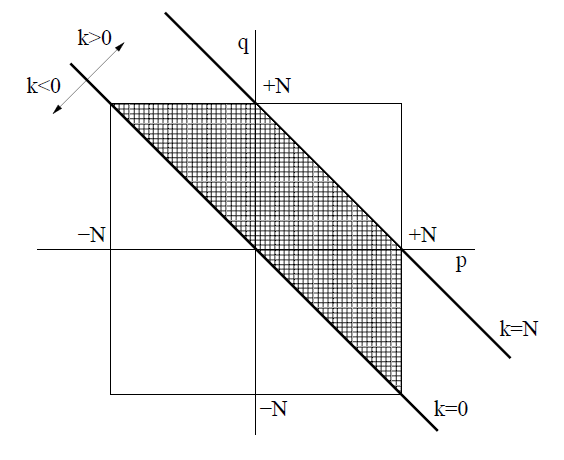
\includegraphics[scale=0.7]{Burgers/Burger}
	\caption{Representation of all the possible interactions between the modes in the convective term. Extracted from \cite{CTTC2014}}
	\label{TriadicFigure}
\end{figure}
In Fourier space $\bar{û}_{-k}=û_{k}$, so only the positive modes need to be solved. Moreover, since the Fourier series are truncated for $k\leq|N|$, the only possible interactions are those of $p+q\leq N$. Therefore, only the interactions between the lines $k=0$ and $k=+N$ have to be considered in the computation of the convective term.

\section{Discretization}
In order to solve the equation it is necessary to discretize it over time. The time-integration scheme used is the fully explicit one:
\begin{equation}
\frac{û_{k}^{n+1}-û_{k}^{n}}{\Delta t}+\sum_{p+q=k}û_{q}iqû_{q}=-\frac{k^{2}}{Re}û_{k}+F_{k}
\end{equation}
However, the time step needs to be small enough to guarantee good results. A CFL-like condition is imposed:
\begin{equation}
\Delta t\leq C_{1}\frac{Re}{N^{2}}
\end{equation}

\subsection{Large-Eddy Simulation}
The method proposed in the previous lines is called Direct Numerical Simulation (DNS), and it does not provide as good results as other methods based on some turbulence models. A method that can improve the calculations is the Large-Eddy Simulation (LES). Like the DNS, it starts with a one-dimensional equation in which the unknown is not the velocity but its average.
\begin{equation}
\frac{\partial\bar{u}}{\partial t}+\bar{u}\frac{\partial\bar{u}}{\partial x}=\frac{1}{Re}\frac{\partial^{2}\bar{u}}{\partial x^{2}}+f-\frac{\partial}{\partial x}\tau\left(u\right)
\end{equation}
where
\begin{equation}
\tau\left(u\right)=\bar{u^{2}}-\bar{u}^{2}
\end{equation}
In the Smagorinsky model, this subfilter tensor is modeled using a viscosity called the eddy-viscosity:
\begin{equation}
\tau\left(u\right)\approx\nu_{t}\frac{\partial\bar{u}}{\partial x}
\end{equation}
Smagorinsky also obtained an expression for $\nu_{t}$, but it cannot be applied in Fourier space. To do so, a spectral viscosity model is used:
\begin{equation}
\nu_{t}\left(k/k_{N}\right)=\nu_{t}^{+\infty}\left(\frac{E_{k_{N}}}{k_{N}}\right)^{1/2}\nu_{t}^{*}\left(\frac{k}{k_N}\right)
\end{equation}
where
\begin{equation}
\nu_{t}^{+\infty}=0.31\frac{5-m}{m+1}\sqrt{3-m}C_{K}^{-3/2}
\end{equation}
\begin{equation}
\nu_{t}^{*}\left(\frac{k}{k_{N}}\right)=1+34.5e^{-3.03\left(k_N/k\right)}
\end{equation}
where $m$ is the slope of the energy spectrum, $E_{k_{N}}$ is the energy at the truncated frequency $k_{N}$, and $C_{K}$ is the Kolmogorov constant. With the results obtained with the DNS, it can be deduced that $m=2$ approximately. And for the value of the Kolomogorov constant, it is known that for the one-dimensional Burgers' equation it is $C_{K}\approx0.4523$.